\section{Code Size}

This section looks at the size of the end object files for various Rust libraries and examples.
A comparison with the size of identical programs implemented in C is also included.

Code size is an important factor in an embedded system.
Primarly the system is more restricted than conventional systems exspecially when it comes to storage.
For the EFM32 line of microcontrollers the code is stored in flash memory.
In \autoref{tab:efm32-family} in \autoref{sec:back:hw} we showed that the flash memory in the EFM32 family of microcontrollers ranges from 4kB to 1024kB.
As \autoref{sec:before-main} explains the flash memory should not only contain the program code but also the constant data defined in the program.
This limits the code size even further.

Each program was compiled with optimization levels O0, O1, O2 and O3, the O0 level is compiled both with and without debugging symbols.
Compiling the library results in a lib*.rlib file which is an archive containing object files for the code contained in the library.
Compiling executable programs results in an elf binary file.
The size is then calculated by executing the \emph{arm-none-eabi-gcc} program.

\subsection{Measuring Size}

The \emph{arm-none-eabi-gcc} program accepts an elf binary, an object file or an archive as argument.
The program then reads the file and reports the size of the \textbf{text}, \textbf{data}, \textbf{bss} sections described in \autoref{sec:back:elf}.
If the argument is an archive the program will iterate through all the objects in the archive an report the size for each individual file.

\subsection{Parameters}
\label{sec:size:params}
The programs was generated by setting the \emph{profile} parameters of in the Cargo.toml file, described in \autoref{sec:cargo:profile}.
The parameters used are shown in \autoref{tab:size:params} with their effect.

\begin{table}[H]
  \centering
  \begin{tabular}{|l|l|l|}
    \hline
    Parameter & Values & Effect \\
    \hline
    debug & true, false & sets the \textbf{-g} flag on the compilers  \\
    debug-assertions & true, false & a way to remove assertion statements \\
    opt-level & 0, 1, 2, 3 & sets the optimization flag on the compilers \\
    lto & true, false & sets the Link Time Optimization flag on the linker \\
    \hline
  \end{tabular}
  \caption{Cargo.toml profile parameters and their effect}
  \label{tab:size:params}
\end{table}

Each program in this section is compiled with 5 different settings as given by \autoref{tab:size:settings}.
\begin{table}[H]
  \centering
  \begin{tabular}{|l|l|l|l|l|l|}
    \hline
    & 1     & 2     & 3     & 4     & 5     \\
    \hline
    debug            & true  & false & false & false & false \\
    debug-assertions & true  & false & false & false & false \\
    opt-level        & 0     & 0     & 1     & 2     & 2     \\
    lto              & false & true  & true  & true  & true  \\
    \hline
  \end{tabular}
  \caption{Compilation settings}
  \label{tab:size:settings}
\end{table}

\subsection{Libraries}

This section looks at the code size the REL libraries along with the cmsis and startup libraries.
The REL libraries are all Rust code, while the cmsis and startup libraries contain bindings C code and the actual C code compiled with gcc.
The same compiler options from \autoref{sec:size:params} applies to the C compiler aswell.
As the code size of libraries varies from a few bytes to 400KB the results are presented in two separate figures.
\autoref{fig:size:lib:small} shows the small libraries ranging from 4B to 3KB and \autoref{fig:size:lib:large} shows the large libraries in ranges 100KB to 400KB.

Both figures distinguises between the three sections reported by the \emph{size} program but only the \textbf{text} segment is prominent.
This is because there is not much allocation in the the REL libraries, in fact the only allocation is 8B in the \textbf{data} section of the startup library.

The bars for each library from left to right represents the sizes of programs compiled with different parameters as described in \autoref{tab:size:settings}.
The general trend is that the code size decrease when the optimization level is incresased.

\begin{figure}[H]
  \begin{center}
    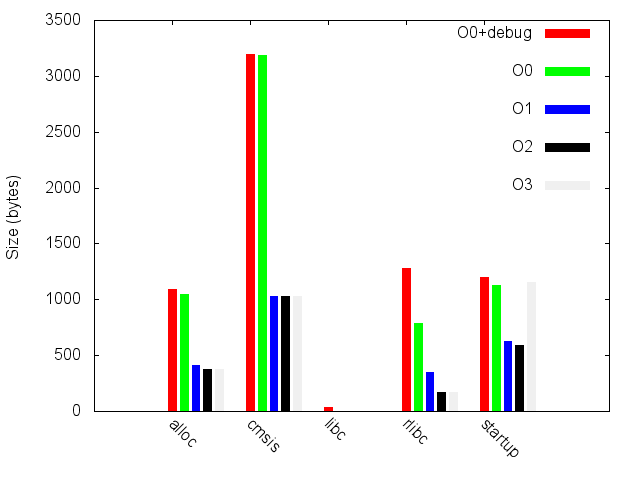
\includegraphics[scale=0.3]{results/plots/size/lib/small/size.png}
  \end{center}
  \caption{Code size for small Rust libraries}
  \label{fig:size:lib:small}
\end{figure}
\begin{figure}[H]
  \begin{center}
    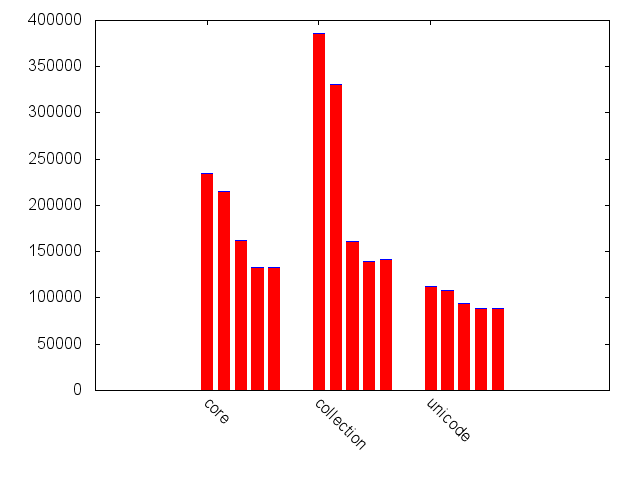
\includegraphics[scale=0.3]{results/plots/size/lib/large/size.png}
  \end{center}
  \caption{Code size for large Rust libraries}
  \label{fig:size:lib:large}
\end{figure}
\todo{do subfigure when oo section lands the packages}

A notable result in \autoref{fig:size:lib:small} is the increase in code size for the startup library when moving from O2 to O3.
This increase of 500B is not in the Rust section of the startup library but the CMSIS Cortex-M3 System Layer provided by Silicon Labs.
We see that the code footprint of the libc implementation is only 4B when compiled with debugging symbols and actually disappears completely when the library is optimized.
This points the fact that Rust delivers a Zero Cost Abstraction when calling C through \emph{ffi} without safe wrappers.
The libc only responsibilty is to expose a few functions and provide type aliases for using C specific datatypes.
All of these are static abstractions and can be removed at compile time.

\autoref{fig:size:lib:large} shows that some of the central libraries in REL are quite large.
An importaint point here is that, although the \emph{core} library by it self is over 100KB, when optimized for a program utilizing the library can be substantially smaller.
This is because of the fact that a library build must provide all the functionality of the source code, while an executable build can eliminate all the functionality of the library that is not used.

By considering the size of the largest and the smallest build for each program we see that the compress factor when applying optimizations is 2.3x on average.

\subsection{Executables}

This subsection consideres the code size of actual runnable programs.
Functinally equivalent versions are written in both Rust and C and here we compare the size of the binaries produced at each optimization level presented in \autoref{tab:size:settings}.
For the C program an additional optimization level, -Os, is given as the rightmost bar.
This level tells the compiler to optimize for code size, it is not available for the Rust compiler at time of writing.
The first figure, \autoref{fig:size:bin:large}, in this section looks at the size of binaries generated for the two projects described in \autoref{sec:projects}.

\begin{figure}[H]
  \begin{center}
    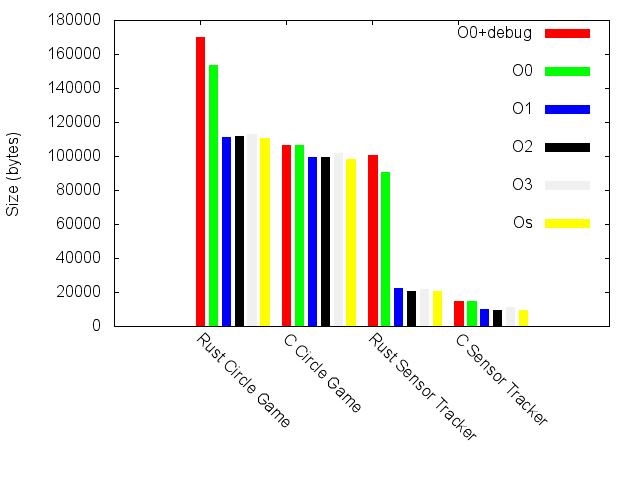
\includegraphics[scale=0.5]{results/plots/size/bin/large/size.png}
  \end{center}
  \caption{Code size for Project binaries}
  \label{fig:size:bin:large}
\end{figure}

The same trend as for the Libraries is seen for the Rust programs, higher optimizations levels provides a smaller binary.
Again we see that the O2 level provides a small size gain over the O3 version.
The compression factor between the larges and smalles binaries is 2.3x on avarage for the Rust code.

The C code does not exibit the same size loss when optimized and the compression factor is 1.3x on average, with Os being the smallest.

\autoref{fig:size:bin:small} shows the code size of a minimal program to boot the Gecko.
Both implementations only contain an infinite loop and are evaluate to illustate the overhead of the languages.

\begin{figure}[H]
  \begin{center}
    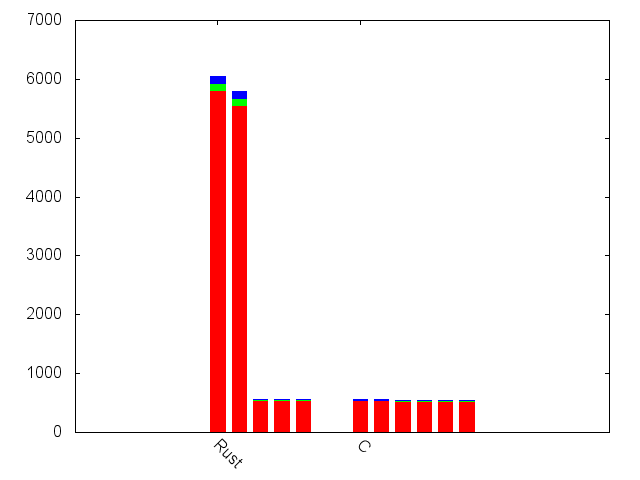
\includegraphics[scale=0.5]{results/plots/size/bin/small/size.png}
  \end{center}
  \caption{Code size for minimal program}
  \label{fig:size:bin:small}
\end{figure}

As explained in \autoref{sec:impl:booting} Rust does not require any aditional initialization or setup compared to C.
This is evendient in \autoref{fig:size:bin:small} where the binaries are the same size when applying optimizations.
The debug and unoptimized Rust build is 10x lager than the optimized versions.

\autoref{tab:size:c-vs-rust} compares the size of the smallest C and Rust binaries shown above.
The number reported is generated by dividing the size of the Rust binary by the size of the C binary giving the factor of witch the Rust version is larger than the C version.

\begin{table}[H]
  \centering
  \begin{tabular}{|c|c|c|}
    \hline
    Circle Game & Sensor Tracker & Minimal Main \\
    \hline
    1.22x & 3.57x & 1.03x \\
    \hline
  \end{tabular}
  \caption{Rust code size relative to C}
  \label{tab:size:c-vs-rust}
\end{table}

We see from \autoref{tab:size:c-vs-rust} that the Rust binaries are on average 1.94x larger than the C binaries, although some of the individual programs comes much closer.

\subsection{Discussion}

This section has shown that the code size of all Rust binaries are larger than their C counterparts.
The optimized Rust builds comes close to C builds with being 1.94x larger on average, while the debug builds are far bigger, 6.88x on average.

The test hardware used to produce the results given here is, as mentioned in \autoref{sec:back:hw}, the EFM32GGF1024.
This chip has 1MB for storing the code and therefore running the debug builds which maxed out at ~176kB was not a problem.

Considering the Minimal Main debug binary presented in \autoref{fig:size:bin:small} and comparing to the chips with lower specifications in the EFM32 family (\autoref{tab:efm32-family}), we see that a debug build can not be executed at small versions of the Zero and Tiny Gecko.
Looking at the Sensor Tracker application even the heavily optimized version of the Rust build can not run on the largest version of the Zero and Tiny Gecko.

Reading the results presented here should take in mind that the comparions are made between a mature production proven compiler \textbf{gcc} and a pre/close to 1.0 compiler \textbf{rustc}.
The design objectives for the 1.0 version of Rust as outlined in \autoref{sec:rust:roadmap} has been on stabilizing the language APIs and features.
This indicates that non-breaking changes like compiler optimizations both for compiler speed and binary code sizes not has been a priority leading up to the 1.0 release.
